%============================== Setting teh Document=============================================

\documentclass[aspectratio=169]{beamer}
\usepackage[italian]{babel} 
\usepackage[utf8]{inputenc} 
\usepackage[T1]{fontenc}
\usepackage{graphicx}
\usepackage{xcolor}
\usetheme{CambridgeUS}
\usepackage{multicol}
\usepackage[pscoord]{eso-pic}
\usepackage{setspace}
\usepackage{tikz}

%==========================Set the foot line========================================================
\makeatletter

\setbeamercolor*{author in head/foot}{parent=palette tertiary}
\setbeamercolor*{title in head/foot}{parent=palette primary}
\setbeamercolor*{date in head/foot}{parent=palette primary}

\setbeamercolor*{section in head/foot}{parent=palette tertiary}
\setbeamercolor*{subsection in head/foot}{parent=palette primary}
% colors for the external link field
\setbeamercolor*{LinkToIndex}{parent=palette tertiary}

\defbeamertemplate*{footline}{}
{
	\leavevmode%
	\hbox{%
		\begin{beamercolorbox}[wd=.25\paperwidth,ht=2.25ex,dp=1ex,center]{author in head/foot}%
			\usebeamerfont{author in head/foot}%\insertsection
		\end{beamercolorbox}%
	
		\begin{beamercolorbox}[wd=.25\paperwidth,ht=2.25ex,dp=1ex,center]{title in head/foot}\centering{-Tel-}\hspace*{2ex}
			%\insertsubsection
		\end{beamercolorbox}%
	
	% this is a new field with an external link
	    \begin{beamercolorbox}[wd=.25\paperwidth,ht=2.25ex,dp=1ex,center]{LinkToIndex}%
	    	\usebeamerfont{author in head/foot}\centering{\href{mailto:f.rombaldoni@campus.uniurb.it}{f.rombaldoni@campus.uniurb.it}}\hspace*{2ex}
    	\end{beamercolorbox}%

		\begin{beamercolorbox}[wd=.25\paperwidth,ht=2.25ex,dp=1ex,center]{date in head/foot}%
			\usebeamerfont{date in head/foot}\centering{Francesco Rombaldoni}\hspace*{2em}
		\end{beamercolorbox}}%	

	\vskip0pt%
}
\setbeamersize{text margin left=1em,text margin right=1em}
\makeatother

\AddToShipoutPictureFG{
	\put(\LenToUnit{.884\paperwidth},
	\LenToUnit{.25\paperheight})
	{\vtop{{\null}
			\makebox{\begin{tikzpicture}
					% << Replace with your personal image >>
					\clip (0,0) circle (6mm) node {
\includegraphics[width=22mm]{Imgs/temp}};
\end{tikzpicture}}}}} 

\setbeamercovered{dynamic}

\title{Offerta Di Ripetizioni} 
\author{Francesco Rombaldoni} 

%===========================================Document starting===============================================
\begin{document}

\section{Riversamenti a prezzi modici}
\setbeamertemplate{navigation symbols}{}
\begin{frame}[t]{\textbf{Riversamenti di materiale analogico in digitale}}
	
	\mbox{
	\colorbox{gray!20}{\begin{minipage}[t][0.8\textheight][t]
			{\dimexpr0.4\textwidth-2\fboxsep-2\fboxrule-5pt\relax}
			\centering{\textbf{\textcolor{red}{Hai anche tu delle videocassette VHS o dei filmini in video 8 che vorresti riversare in digitale?} \newline \textcolor{blue}{Allora stai guardando la locandina giusta!}}
				\newline
				\scriptsize{Sono un informatico appassionato di tecnologia vintage che per riversare i miei contenuti analogici ho acquistato della strumentazione semiprofessionale, se anche te, come me in passato, ti sei reso conto di non aver salvato in digitale i vecchi ricordi, domandandoti ora se li puoi ancora rivedere utilizzando le nuove tecnologie,} \textbf{Non esitare a contattarmi!}
			}
	\end{minipage}}
		\colorbox{gray!20}{\begin{minipage}[t][0.8\textheight][t]
			{\dimexpr0.4\textwidth-2\fboxsep-2\fboxrule-5pt\relax}
		\textbf{Formati supportati}
		{\scriptsize
		\begin{multicols}{3}
		\begin{itemize}
			\item  VHS
			\item VHS-C
			\item Video8
		\end{itemize}
		\end{multicols}}
		\textbf{Supporti di memorizzazione}
		{\scriptsize
		\begin{itemize}
			\item  HDD-USB
			\item Chiavette-USB
			\item Assemblaggio di un multimedia Box da TV che non necesita di un ulteriore telecomando! 
		\end{itemize}}
		\begin{figure}
			\centering
			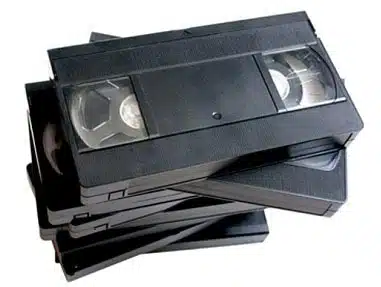
\includegraphics[width=0.57\textwidth]{Imgs/VHS.png}
		\end{figure}
	\end{minipage}}


\colorbox{gray!20}{\begin{minipage}[t][0.8\textheight][t]
		{\dimexpr0.22\textwidth-2\fboxsep-2\fboxrule-5pt\relax}
		\centering{\textbf{Contattami su WhatsApp}}
			\begin{figure}
			\centering
			
\includegraphics[width=0.5\textwidth]{Imgs/WhatsApp-QR-code}
		\end{figure}
		\centering{\textbf{Contattami su Telegram}}
	\begin{figure}
		\centering
		
\includegraphics[width=0.5\textwidth]{Imgs/WhatsApp-QR-code}
	\end{figure}
	\end{minipage}}
}


\end{frame}

\end{document}
